% ===========================================================================
\section{Results}
\label{sec:results}
% ===========================================================================

\subsection{The sector}

Pakistani households emitted \SI{24.22}{\mega\tonne} \COe{} in FY2023--24 on AR5 metrics
under the reference (\SI{29.47}{} under configuration~L; Table~\ref{tab:configs}), or
\SI{24.06}{\mega\tonne} on AR6, plus \SI{65359}{\giga\gram} of biogenic \COtwo{} reported
as a memo item outside the national total. This subsection's detail tables ride the
reference; every headline is restated under configuration~L in
Table~\ref{tab:configs}.

\begin{table}[htbp]
\centering
\footnotesize
\begin{tabular}{@{}llrrr@{}}
\toprule
\textbf{Stream} & \textbf{Gas} & \textbf{Gg} & \textbf{Mt \COe{}} & \textbf{$\pm$\%} \\
\midrule
Natural gas & \COtwo{}  & 15\,963.42 & 15.963 &  10.8 \\
            & \CHfour{} &      1.42 &  0.043 & 150.3 \\
LPG         & \COtwo{}  &  2\,142.15 &  2.142 &  20.9 \\
Kerosene    & \COtwo{}  &      77.57 &  0.078 &  20.2 \\
Coal        & \COtwo{}  &      32.27 &  0.032 &  40.3 \\
Generators  & \COtwo{}  &     172.93 &  0.173 &  40.2 \\
Dung cake   & \CHfour{} &      38.05 &  1.065 & 154.0 \\
            & \NtwoO{}  &       0.51 &  0.134 & 154.0 \\
Firewood    & \CHfour{} &     108.26 &  3.031 & 154.0 \\
            & \NtwoO{}  &       1.44 &  0.383 & 154.0 \\
Crop resid. & \CHfour{} &      36.70 &  1.027 & 161.6 \\
            & \NtwoO{}  &       0.49 &  0.130 & 161.6 \\
\midrule
\textbf{Total} & & & \textbf{24.222} & \textbf{22.9} \\
\bottomrule
\end{tabular}
\caption{Residential fuel combustion, FY2023--24, AR5. Minor gas rows below
\SI{0.01}{\mega\tonne} are omitted from the table and included in the total. Biomass \COtwo{}
is a memo item and does not appear. The total's $\pm$\SI{22.9}{\percent} combines the rows
as if independent; the sector's primary figure is the grouped Approach-1
$\pm$\SI{23.1}{\percent}, which shares each stream's activity term across its gas rows, and
the national Monte Carlo counterpart is $\pm$\SI{30.4}{\percent}. The last is wider for a
named reason: at parameter level the eight biomass CH\textsubscript{4} and
N\textsubscript{2}O rows' declared widths are superseded by the widths their named factor
and calorific-value parameters imply (\texttt{data/uncertainty\_reconciliation.csv}, the
rc41 dispositions), and mean-preserving lognormal draws skew wider still; all are the same
decomposition under different treatments, not competing estimates.}
\label{tab:results}
\end{table}

\begin{figure}[htbp]
\centering
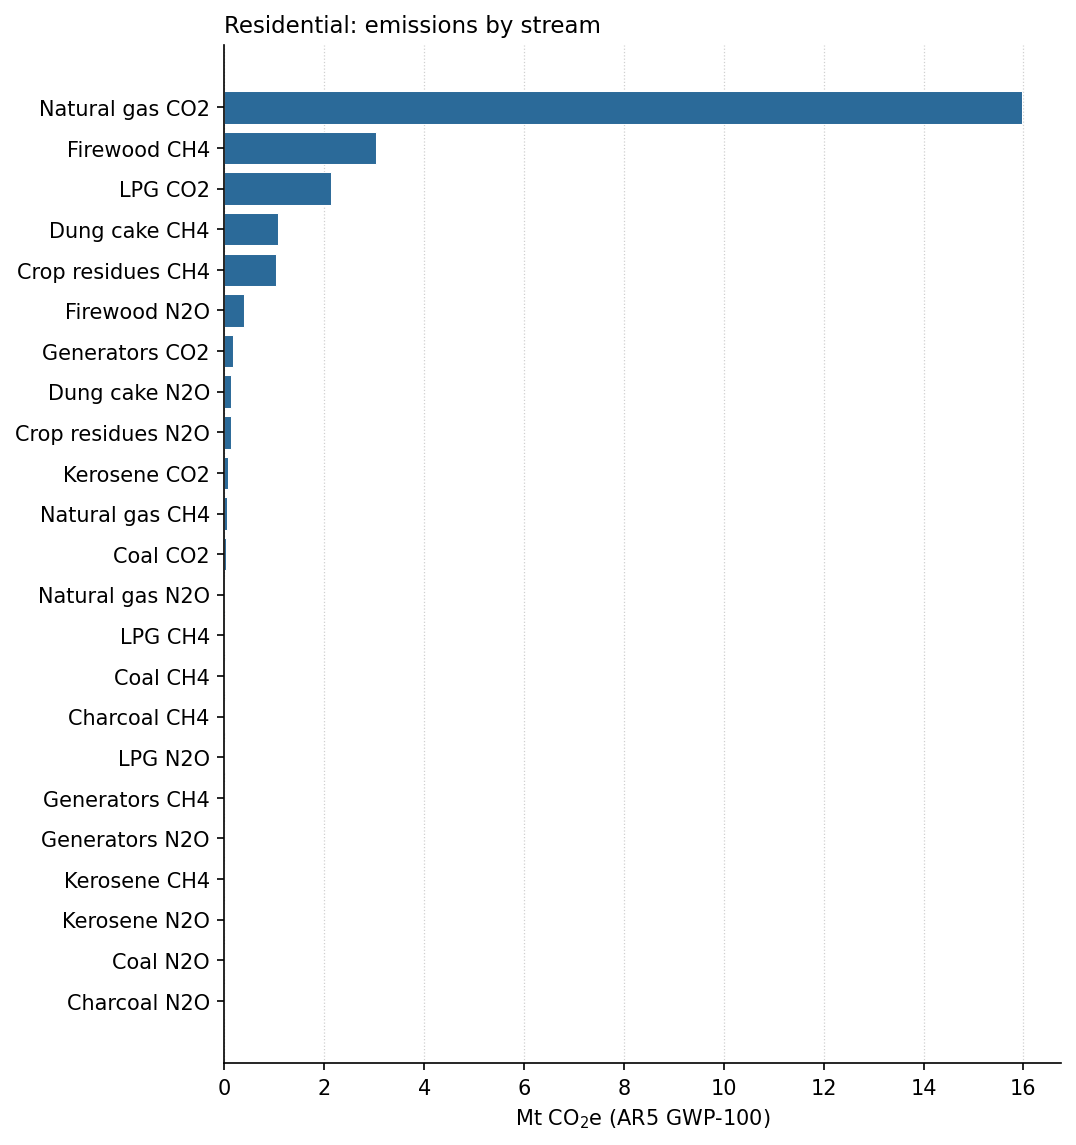
\includegraphics[width=\linewidth]{residential_streams.png}
\caption{Emissions by stream and gas. Biomass streams appear here through their \CHfour{} and
\NtwoO{} only, which is why natural gas carries a far larger share of the emissions than of the
energy.}
\label{fig:streams}
\end{figure}

The inversion between energy and emissions is the central arithmetic result. Biomass supplies
\SI{65.4}{\percent} of household energy and \SI{24}{\percent} of reported emissions; natural
gas supplies \SI{30.5}{\percent} of the energy and \SI{66}{\percent} of the emissions. This is
the biomass memo convention working as intended, and it is why a household-energy statistic and
a household-emissions statistic for Pakistan tell opposite stories about which fuel matters.

\subsection{Firewood, and what it is worth}

\begin{table}[htbp]
\centering
\footnotesize
\begin{tabular}{@{}lr@{}}
\toprule
\textbf{Case} & \textbf{Mt \COe{}} \\
\midrule
Firewood excluded entirely & 20.808 \\
Firewood quantity $-35\%$  & 23.027 \\
Reported                   & 24.222 \\
Firewood quantity $+35\%$  & 25.416 \\
\bottomrule
\end{tabular}
\caption{The sector reported four ways across the firewood cases. Firewood is
survey-anchored since the HIES re-anchoring; the exclusion case bounds what the stream is
worth, and the dung configurations---a larger structural axis---are treated below.}
\label{tab:sensitivity}
\end{table}

\begin{figure}[htbp]
\centering
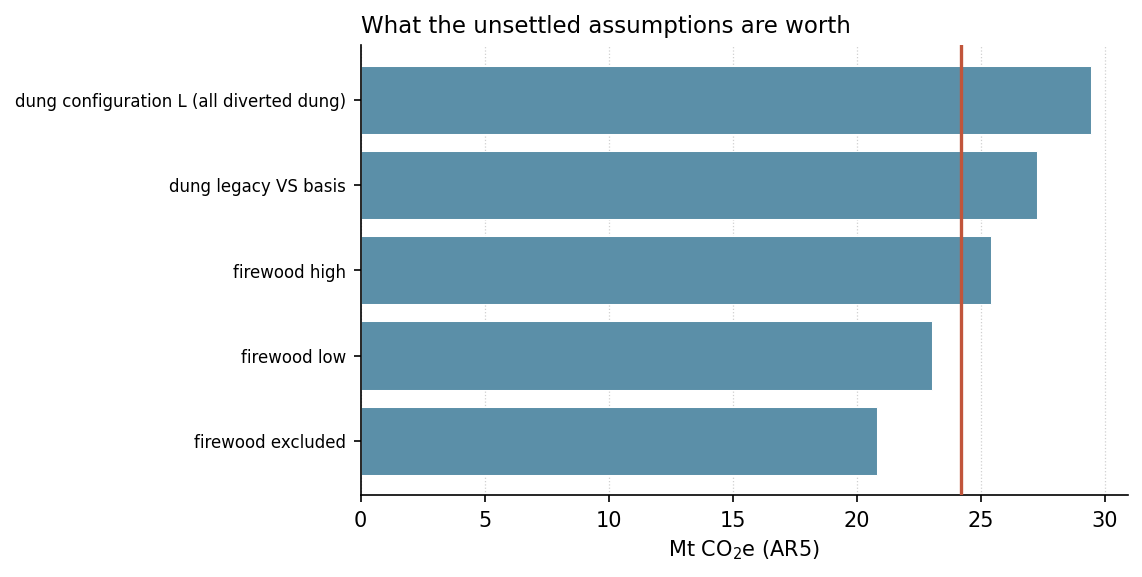
\includegraphics[width=\linewidth]{residential_sensitivity.png}
\caption{The published sensitivity rows as a range around the reported figure. From
lowest to highest: firewood excluded entirely (\SI{20.81}{}), the HIES firewood
quantity $-35\%$ (\SI{23.03}{}) and $+35\%$
(\SI{25.42}{}), the superseded legacy VS dung basis
(\SI{27.28}{}), which is a reading of configuration~L, and configuration~L itself
(\SI{29.47}{\mega\tonne}); the vertical line marks the reference at
\SI{24.22}{\mega\tonne}.}
\label{fig:sensitivity}
\end{figure}

Dropping firewood entirely moves the sector by \SI{14}{\percent}---from \SI{24.22}{} to
\SI{20.81}{\mega\tonne}---which is less than a reader might expect for a fuel supplying
\SI{39}{\percent} of household energy, and the reason is again the memo convention: only
firewood's methane and nitrous oxide are in the total. What exclusion \emph{would} remove is
\SI{40418}{\giga\gram} of biogenic \COtwo{} from the memo and a comparable share of the
air-pollutant layer, where firewood matters most.

\subsection{The survey against the controls}

\begin{table}[htbp]
\centering
\footnotesize
\begin{tabular}{@{}llrrl@{}}
\toprule
\textbf{Fuel} & \textbf{Role} & \textbf{HIES 2024--25} & \textbf{Engine} & \textbf{Ratio} \\
\midrule
Firewood (Mt)   & primary     & 23.13 & 23.13 & 0.94$^b$ \\
Dung cake (Mt)$^c$ & primary  & 10.93 & 58.74 & 0.186 \\
LPG (Mt)        & diagnostic  &  0.90 &  0.72 & 1.248 \\
Kerosene (ML)   & diagnostic  & 77.96 & 30.79 & unusable$^a$ \\
\bottomrule
\end{tabular}
\caption{The published survey-versus-control comparison
(\texttt{residential\_hies\_comparison\_2024.csv}, abridged). Diagnostic ratios are
published and never applied. $^a$The kerosene item rides 116 outlier-heavy households
whose implied unit value is a fifth of retail. $^b$Against FAOSTAT's moisture-matched
equivalent; the survey IS the estimate. $^c$The survey series at the reference year (the
per-household quantity interpolated between the two rounds; the 2024--25 round as
measured is \SI{11.97}{\mega\tonne}) against the dung agriculture diverts, not against
an engine control: the survey IS the estimate, and the ratio is the part of the diverted
supply households are observed burning.}
\label{tab:hies}
\end{table}

The diverted supply is $r_{\text{dung}} = 4.90$ times what households reported in the
2024--25 round, and \num{5.4} times the survey series at the reference year: the nitrogen
ledger implies
\SI{58.7}{\mega\tonne} of air-dry cake, and the survey series puts \SI{10.9}{} in
households. Mass
conservation constrains what agriculture diverted; it is not evidence about the
destination of the conserved mass, and the correct identity is
$D_{\text{diverted}} = D_{\text{residential}} + D_{\text{other/unresolved}}$, not
$D_{\text{diverted}} = D_{\text{residential}}$. The residential row measures what
households burn, and the survey is what observes it; the ledger's burned-fuel shares are
unmeasured Tier~2 values, and nothing held supports a fivefold survey under-count. The
reference is therefore the survey-observed residential-demand configuration
(S), which books the household consumption the survey measures and leaves the
residual's destination unresolved, outside the total. Configuration L, in which the
full diverted quantity is booked to households, was the reference of earlier releases
and is retained beside it as a destination assumption for the diverted dung, not a
reading of household use. The survey is not settled either: it sees only in-scope
household consumption of formed cake, its two rounds disagree by a factor of
\num{1.53} per household, and in 2024--25 the top 5\% of reporting households hold
\SI{44.7}{\percent} of the reported dung (Section~\ref{sec:data}).

\subsection{The reference and configuration L}

\begin{table}[htbp]
\centering
\footnotesize
\begin{tabular}{@{}lrr@{}}
\toprule
 & \textbf{L (all diverted)} & \textbf{S (survey, reference)} \\
\midrule
Dung cake, air-dry (Mt)        & 58.74 & 10.93 \\
Household energy (TJ)          & 1\,487\,257 & 932\,675 \\
Sector \COe{}, AR5 (Mt)        & 29.468 & 24.222 \\
Biogenic memo \COtwo{} (Gg)    & 120\,817 & 65\,359 \\
Primary \PM{} (kt)             & 632.0 & 282.8 \\
Black carbon (kt)              & 41.5  & 20.0 \\
Ratio vs road exhaust \PM{}    & 109.4 & 49.0 \\
National share (\%)            & 6.55  & 5.45 \\
\bottomrule
\end{tabular}
\caption{Every headline quantity under both dung configurations
(\texttt{residential\_configurations\_2024.csv}). S is the reference, and the
detailed spatial and temporal layers are presented under it;
under S, \SI{47.8}{\mega\tonne} of diverted air-dry cake has no observed
destination and is carried as unresolved, outside the total---candidates include
commercial tandoors and eateries, non-household
burning, over-stated burned-fuel shares in the manure-management configuration, field
application, and
survey undercapture of own-produced cake.}
\label{tab:configs}
\end{table}

The configuration choice is the dominant structural axis of the sector: leaving
configuration L for the reference lowers the
total by \SI{5.25}{\mega\tonne}, the particulate headline by more than a factor of two,
and the road-transport ratio from \num{109} to \num{49}. The configurations describe alternative material destinations rather than
a probability interval. Section~\ref{sec:validation} shows the one
external anchor that speaks to it: at the matched year, configuration S sits within
\SI{15}{\percent} of the CCAC/SEI assessment's implied residential particulate, while L
is \num{2.6} times above it.

The \SI{47.8}{\mega\tonne} left unresolved under the reference holds
\SI{1025.6}{\kilo\tonne} of nitrogen and carries no emission. Its candidate
destinations are priced one at a time beside the national total, with no probability
attached (\texttt{national\_dung\_variants.csv}): burned by non-household users,
\SI{5.25}{\mega\tonne} more, which is configuration L reclassified; returned to manure
management, \SI{4.54}{} more; applied to fields, \SI{3.04}{} more.

\subsection{Ten fiscal years and monthly allocation}

The sector reports FY2015--16 through FY2024--25: \SI{21.5}{} to
\SI{22.7}{\mega\tonne}, growth carried by gas connections and the survey-anchored biomass streams, with each
stream's basis recorded with the product. Gas uses nine reported OGRA annual controls
\citep{ograarchive}, including the full FY2024--25 edition, and one labelled
interpolation across the ten-year panel; minor fuel streams remain held. The
matched calendar years this series unlocks are what Section~\ref{sec:validation}'s
official comparisons stand on. For the detailed FY2023--24 reference, a synthetic-labelled monthly layer on
measured degree-days \citep{nasapower} produces a pronounced winter peak that coincides
with Pakistan's smog season---January at \SI{49}{\kilo\tonne} of \PM{} per month
against July's \SI{16}{}---with the generator stream alone running the opposite season
against summer load-shedding. These are allocations of the annual total, not monthly
observations; the output carries the base-load and climate-load components separately,
so the degree-day shape is auditable against the flat cooking term it never touches.

\subsection{Provincial allocation}

\begin{figure}[htbp]
\centering
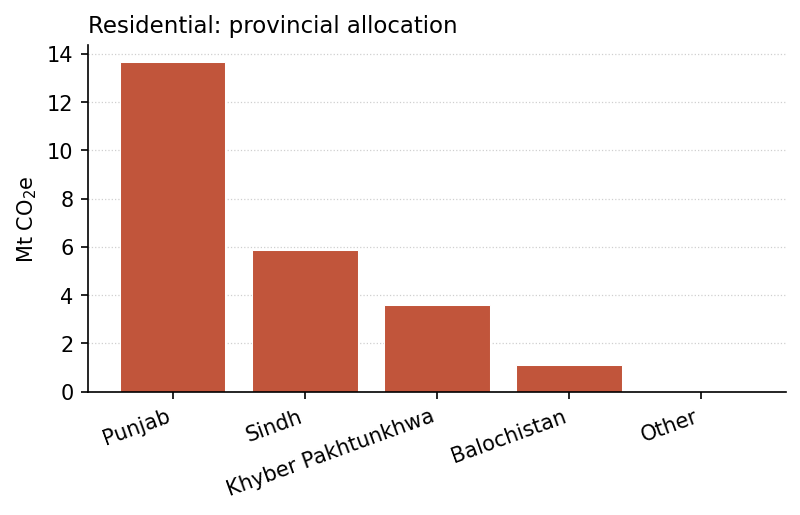
\includegraphics[width=\linewidth]{residential_provincial.png}
\caption{Punjab \SI{13.69}{\mega\tonne}, Sindh \SI{5.86}{\mega\tonne}, Khyber Pakhtunkhwa
\SI{3.58}{\mega\tonne}, Balochistan \SI{1.09}{\mega\tonne}. Each stream rides its own proxy;
the allocation reconciles exactly against each stream's national figure.}
\label{fig:provincial}
\end{figure}

The pattern broadly follows population, as expected for a household sector, with Sindh
somewhat elevated relative to its population share because piped gas connection rates in
Karachi are high and piped gas is the stream whose \COtwo{} is reportable.

\subsection{Districts and the grid}

Below the provinces, each stream's total splits urban/rural by the survey's own rates
and spreads over \num{134} allocation units by the matching population: named
four-province districts and one grouped Other residual for GB/AJK/ICT. These are
allocation units rather than individually observed districts across all territories.
The agricultural account has \num{116} four-province districts plus its grouped Other
unit. The residential summaries reconcile
per province and stream (\texttt{residential\_district\_2024.csv}); Lahore leads at
\SI{2.13}{\mega\tonne} because gas is urban, with Faisalabad (\SI{1.01}{}) and
Rawalpindi (\SI{0.92}{}) behind it. The grid places the same totals at
\SI{0.05}{\degree} on per-stream surfaces, again exactly reconciled
(Figures~\ref{fig:districtmap} and~\ref{fig:gridmap}). These are allocations, not
observations---no district fuel survey exists---and the within-region split stays
population-shaped until the census cooking-fuel tables land
(Section~\ref{sec:methods}).

\begin{figure}[htbp]
\centering
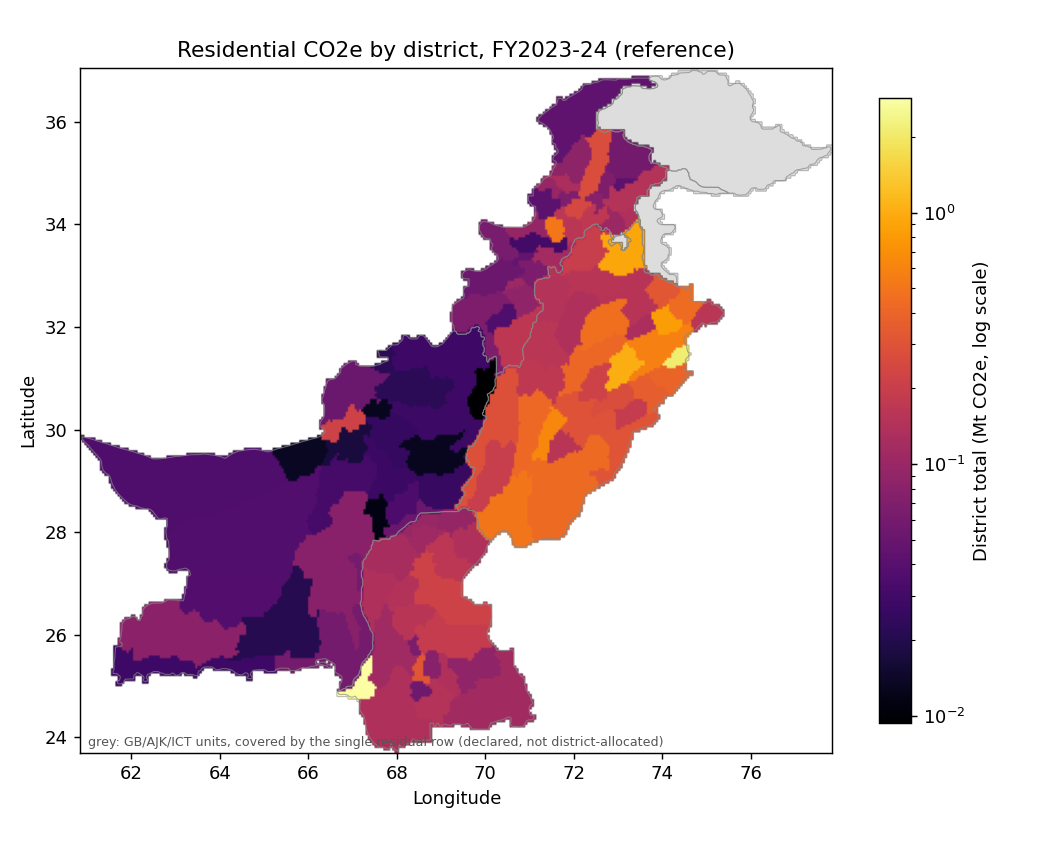
\includegraphics[width=\linewidth]{residential_district_map.png}
\caption{District allocation of residential \COe{} (reference). Each district is
painted with its allocated total; the survey's urban/rural rates on census populations
do the within-province work. The map now resolves every name through the canonical
ADM2 crosswalk: \num{114} of the \num{126} boundary polygons are painted (a polygon
carrying several census units---Karachi's seven, the Chitral and Kohistan splits---paints
their sum), and the \num{12} grey polygons are the GB/AJK/ICT units covered by the
single residual row, a declared class rather than a matching failure; every polygon's
disposition is a row of
\texttt{outputs/residential\_district\_map\_audit\_2024.csv}.
The map is presentation; the CSV is the product.}
\label{fig:districtmap}
\end{figure}

\begin{figure}[htbp]
\centering
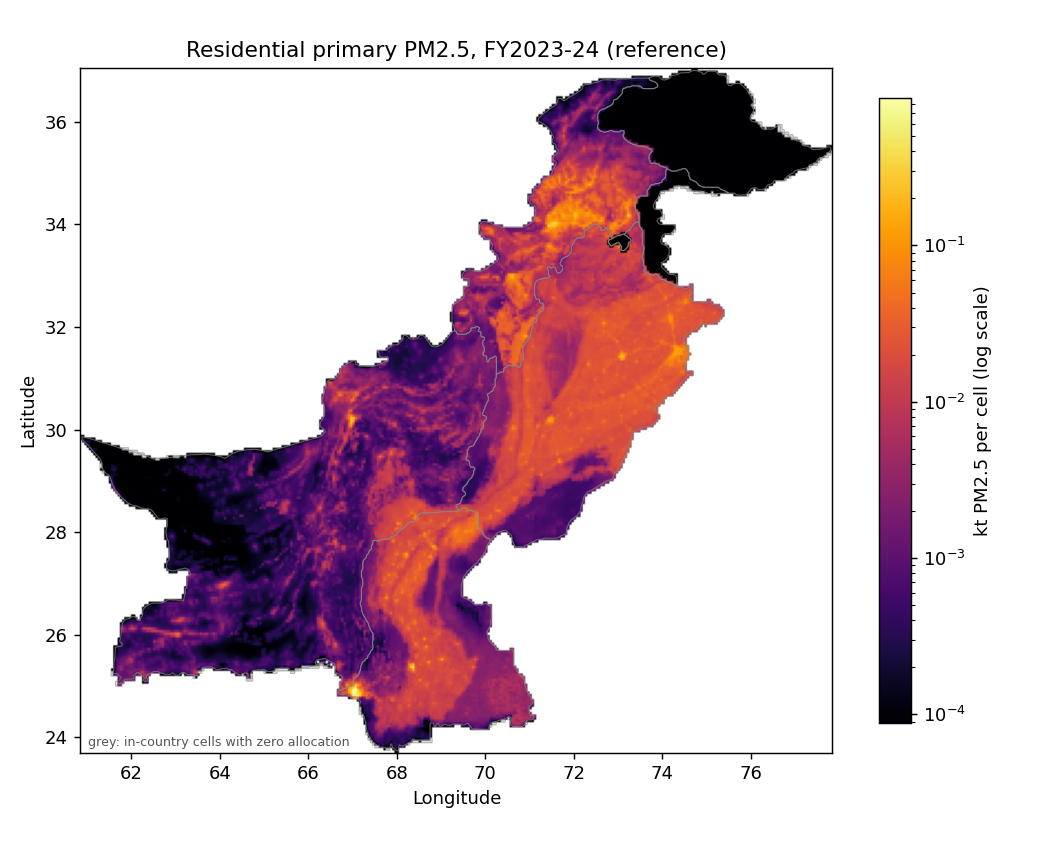
\includegraphics[width=\linewidth]{residential_map_pm25.png}
\caption{Gridded residential primary \PM{} at \SI{0.05}{\degree} (reference):
gas and generators on built-up fraction (ESA WorldCover v200~2021 class~50, CC~BY~4.0,
aggregated from \SI{10}{\metre}---a 2021 surface against FY2023--24 activity, a
declared vintage offset, hashed and documented in
\texttt{data/gis/PROXY\_SOURCES.md}), dung on livestock density, residues on
cropland, the rest on population---declared judgement, exactly reconciled to every
province and stream total. Colour is logarithmic; light grey marks in-country cells with
zero allocation (no proxy weight in that cell), distinct from the white outside the
country boundary.}
\label{fig:gridmap}
\end{figure}

\subsection{Contribution to the national inventory}

Residential fuel combustion is \SI{5.45}{\percent} of Pakistan's national emissions and
\SI{1.27}{\percent} of national Approach-1 variance---a sector whose variance share is
below its level share.

It is also almost unaffected by the cross-sector correlated-factor scenario---which,
since the common-random-numbers rebuild, moves no sector's band, transport's included:
$\pm\SI{30.4}{\percent}$ with parameters shared within the module against
$\pm\SI{30.3}{\percent}$ with factors correlated across sectors in the national Monte
Carlo (the sampled counterparts of the analytic $\pm\SI{23.1}{\percent}$ grouped figure
above). The reason is structural and worth stating as an internal check. That scenario
correlates the shared IPCC fuel-carbon factors across sectors, and this sector's uncertainty is
dominated by biomass \CHfour{} and \NtwoO{} factors that no other sector shares. A sector that
moved materially under it would indicate a factor being shared where it should not be.
